\section{Auswertung} 

\subsection{Das Emissionsspektrum de Cu-Röntgenröhre}

\begin{flushleft}
    Im Folgenden wird das Kupferrmissionsspektrum analysiert. 
    Dazu wird ein Diagramm, Abbildung \ref{Abbildung3} erstellt, die aus den Wertepaaren der Tabelle \ref{Tabelle1} bestehen. 
    Die Integrationszeit pro Winkel liegt bei $t = 10\,\unit{\second}$ und wird in $0.1\unit{\degree}$ Schritten gemessen.
\end{flushleft}

\begin{table}[H]    
    \centering
    \caption{Wertepaare des Kupferemissionsspektrums}
    \label{Tabelle1}
    \begin{tabular} {c  c| c  c| c  c| c  c}
        \toprule
        {$ \theta \mathbin{/} \unit{\degree}$} &
        {$ N $} &
        {$ \theta \mathbin{/} \unit{\degree} $} &
        {$ N $} &
        {$ \theta \mathbin{/} \unit{\degree} $} &
        {$ N $} &
        {$ \theta \mathbin{/} \unit{\degree}$} &
        {$ N $} \\
        \midrule
        11.8 & 400.0 & 15.8 & 234.0 & 19.9 & 182.0  & 24.0 & 105.0 \\
        11.9 & 383.0 & 15.9 & 231.0 & 20.0 & 291.0  & 24.1 & 106.0 \\
        12.0 & 389.0 & 16.0 & 215.0 & 20.1 & 1127.0 & 24.2 & 107.0 \\
        12.1 & 382.0 & 16.1 & 217.0 & 20.2 & 1599.0 & 24.3 & 95.0  \\
        12.2 & 372.0 & 16.2 & 227.0 & 20.3 & 1533.0 & 24.4 & 94.0  \\
        12.3 & 376.0 & 16.3 & 214.0 & 20.4 & 1430.0 & 24.5 & 100.0 \\
        12.4 & 385.0 & 16.4 & 217.0 & 20.5 & 1267.0 & 24.6 & 91.0  \\
        12.5 & 384.0 & 16.5 & 210.0 & 20.6 & 425.0  & 24.7 & 85.0  \\
        12.6 & 382.0 & 16.6 & 211.0 & 20.7 & 241.0  & 24.8 & 88.0  \\
        12.7 & 373.0 & 16.7 & 206.0 & 20.8 & 225.0  & 24.9 & 83.0  \\
        12.8 & 376.0 & 16.8 & 205.0 & 20.9 & 192.0  & 25.0 & 85.0  \\
        12.9 & 373.0 & 16.9 & 198.0 & 21.0 & 188.0  \\
        13.0 & 375.0 & 17.0 & 203.0 & 21.1 & 172.0  \\
        13.1 & 366.0 & 17.1 & 199.0 & 21.2 & 168.0  \\
        13.2 & 354.0 & 17.2 & 198.0 & 21.3 & 169.0  \\
        13.3 & 341.0 & 17.3 & 191.0 & 21.4 & 166.0  \\
        13.4 & 326.0 & 17.4 & 192.0 & 21.5 & 170.0  \\
        13.5 & 318.0 & 17.5 & 184.0 & 21.6 & 174.0  \\
        13.6 & 305.0 & 17.6 & 191.0 & 21.7 & 164.0  \\
        13.7 & 296.0 & 17.7 & 188.0 & 21.8 & 180.0  \\
        13.8 & 286.0 & 17.8 & 181.0 & 21.9 & 179.0  \\
        13.9 & 285.0 & 17.9 & 185.0 & 22.0 & 191.0  \\
        14.0 & 274.0 & 18.0 & 184.0 & 22.1 & 232.0  \\
        14.1 & 264.0 & 18.1 & 179.0 & 22.2 & 300.0  \\
        14.2 & 266.0 & 18.2 & 180.0 & 22.3 & 536.0  \\
        14.3 & 270.0 & 18.3 & 166.0 & 22.4 & 4128.0 \\
        14.4 & 255.0 & 18.4 & 173.0 & 22.5 & 5050.0 \\
        14.5 & 255.0 & 18.5 & 167.0 & 22.6 & 4750.0 \\
        14.6 & 260.0 & 18.6 & 169.0 & 22.7 & 4571.0 \\
        14.7 & 251.0 & 18.7 & 160.0 & 22.8 & 4097.0 \\
        14.8 & 250.0 & 18.8 & 159.0 & 22.9 & 901.0  \\
        14.9 & 248.0 & 18.9 & 157.0 & 23.0 & 244.0  \\
        15.0 & 253.0 & 19.0 & 149.0 & 23.1 & 179.0  \\
        15.1 & 257.0 & 19.1 & 153.0 & 23.2 & 151.0  \\
        15.2 & 248.0 & 19.2 & 150.0 & 23.3 & 145.0  \\
        15.2 & 248.0 & 19.3 & 147.0 & 23.4 & 130.0  \\
        15.3 & 242.0 & 19.4 & 150.0 & 23.5 & 121.0  \\
        15.4 & 249.0 & 19.5 & 148.0 & 23.6 & 126.0  \\
        15.5 & 246.0 & 19.6 & 149.0 & 23.7 & 117.0  \\
        15.6 & 252.0 & 19.7 & 143.0 & 23.8 & 112.0  \\
        15.7 & 236.0 & 19.8 & 153.0 & 23.9 & 110.0  \\
        \bottomrule
    \end{tabular} 
\end{table}

\begin{figure}[H] 
    \centering
    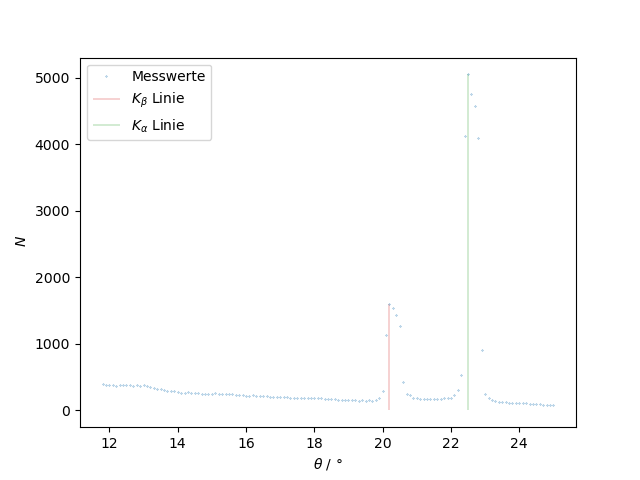
\includegraphics[height=80mm]{bilder/Kupfer.png}
    \caption{Die Abbildung des Kupferemissionsspektrums.\label{Abbildung3} }
\end{figure}

\begin{align}
    \intertext{Die charakteristische Strahlung der $K_{\alpha}$ und $K_{\beta}$ Linie sind bei $\theta_{\text{\alpha}} = 22.5\unit{\degree}$ sowie $\theta{\text{\beta}} = 20.2\unit{\degree}$ sichtlich.
    Die jeweiligen Energien werden durch die Formel}
    E = \frac{h \cdot c}{2 \cdot d \cdot \sin{\theta}}
    \intertext{berechnet. 
    Dabei wird der Ablesefehler des Winkels auf $\increment\theta = 0.1\unit{\degree} = 0.0017\, \text{rad}$ geschätzt.
    Daraus folgt für die Energien}
    E_{K_{\alpha}} = ( 7945.06 \pm 19.43 )\,\text{eV} \notag\\
    E_{K{\beta}} = ( 8805.26 \pm 24.24 )\,\text{eV}. \notag
\end{align}

\subsection{Bestimmung Transmission und der dadurch folgenden Compton-Wellenlänge}

\begin{flushleft}
    Im zweiten Teil wurde die Zählrate der Röntgenstrahlung mit Aluminium-Absorber ($N_{\text{Al}}$) und ohne Aluminium-Absorber ($N_{0}$) in $\increment\alpha = 0.1\unit{\degree}$ Schnitten gemessen. 
    Die Integrationszeit pro Winkel beträgt dabei $t = 200\,\unit{\second}$. 
    Die Anzahl der Röntgenquanten ergibt sich durch $N\* = N \cdot \increment t$ sowie die Messunsicherheit $\increment N = \sqrt{N}$. 
\end{flushleft}

\begin{table}[H]    
    \centering
    \caption{Messdaten der Röntgenröhre mit und ohne Aluminiumabsorber}
    \label{Tabelle2}
    \begin{tabular} {c  c|| c  c  c||  c  c  c}
        \toprule
        {$ \alpha \mathbin{/} \unit{\degree}$} &
        {$ \lambda \mathbin{/} \unit{\pico\meter}$} &
        {$ N_{0} \mathbin{/} \frac{\text{Imp}}{s} $} &
        {$ N^{*}_{0} $} &
        {$ \increment N^{*}_{0} $} &
        {$ N_{\text{Al}} \mathbin{/} \frac{\text{Imp}}{s} $} &
        {$ N^{*}_{\text{Al}}$} &
        {$ \increment N^{*}_{\text{Al}} $} \\
        \midrule
        7.0  & 49 & 226.0 & 45200 & 212.60 & 113.5 & 22700 & 150.67 \\ 
        7.1  & 50 & 232.0 & 46400 & 215.41 & 112.0 & 22400 & 149.67 \\ 
        7.2  & 50 & 240.5 & 48100 & 219.32 & 112.0 & 22400 & 149.67 \\ 
        7.3  & 51 & 248.0 & 49600 & 222.71 & 113.5 & 22700 & 150.67 \\ 
        7.4  & 52 & 255.0 & 51000 & 225.83 & 115.0 & 23000 & 151.66 \\  
        7.5  & 53 & 262.0 & 52400 & 228.91 & 113.5 & 22700 & 150.67 \\  
        7.6  & 53 & 269.0 & 53800 & 231.95 & 113.0 & 22600 & 150.33 \\  
        7.7  & 54 & 276.0 & 55200 & 234.95 & 114.5 & 22900 & 151.33 \\ 
        7.8  & 55 & 281.0 & 56200 & 237.07 & 114.0 & 22800 & 151.00 \\  
        7.9  & 55 & 289.0 & 57900 & 240.62 & 112.0 & 22400 & 149.67 \\  
        8.0  & 56 & 295.0 & 59000 & 242.90 & 109.5 & 21900 & 147.99 \\  
        8.1  & 57 & 300.0 & 60000 & 244.95 & 109.0 & 21800 & 147.65 \\ 
        8.2  & 57 & 308.5 & 61700 & 248.39 & 108.0 & 21600 & 146.97 \\ 
        8.3  & 58 & 311.0 & 62200 & 249.40 & 106.0 & 21200 & 145.60 \\ 
        8.4  & 59 & 317.0 & 63400 & 251.79 & 104.5 & 20900 & 144.57 \\ 
        8.5  & 60 & 324.0 & 64800 & 254.56 & 101.5 & 20300 & 142.48 \\ 
        8.6  & 60 & 328.5 & 65700 & 256.32 & 100.0 & 20000 & 141.42 \\ 
        8.7  & 61 & 332.5 & 66500 & 257.88 & 100.5 & 20100 & 141.77 \\ 
        8.8  & 62 & 337.0 & 67400 & 259.62 &  97.5 & 19500 & 139.64 \\ 
        8.9  & 62 & 340.5 & 68100 & 260.96 &  95.0 & 19000 & 137.84 \\ 
        9.0  & 63 & 348.0 & 69600 & 263.82 &  95.5 & 18500 & 136.01 \\ 
        9.1  & 64 & 350.0 & 70000 & 264.58 &  89.5 & 17900 & 133.79 \\ 
        9.2  & 64 & 353.0 & 70600 & 265.71 &  88.0 & 17600 & 132.66 \\ 
        9.3  & 65 & 356.5 & 71300 & 267.02 &  84.5 & 16900 & 130.00 \\ 
        9.4  & 66 & 359.0 & 71800 & 267.96 &  83.0 & 16900 & 128.84 \\ 
        9.5  & 66 & 363.5 & 72700 & 269.63 &  81.0 & 16200 & 127.28 \\ 
        9.6  & 67 & 367.0 & 73400 & 270.92 &  78.5 & 15700 & 125.30 \\ 
        9.7  & 68 & 369.0 & 73800 & 271.66 &  76.0 & 15200 & 123.29 \\ 
        9.8  & 69 & 370.5 & 74100 & 272.21 &  74.0 & 14800 & 121.66 \\ 
        9.9  & 69 & 375.0 & 75000 & 273.86 &  72.0 & 14400 & 120.00 \\ 
        10.0 & 70 & 375.5 & 75100 & 274.04 &  68.5 & 13700 & 117.05 \\ 
        \bottomrule
    \end{tabular} 
\end{table}

\begin{align*}
    \intertext{Zudem wird eine Totzeitkorrektur nach der Gleichung [...] vorgenommen, unter der Beachtung von einer Totzeit von $\eta = 90\,\unit{\micro\second}$. 
    Dazu wird die Zählrate $I$ und die Transmission $T$, welche sich durch $T = \frac{I_{\text{Al}}}{I_{0}}$ berechnen lässt, tabellarisch eingetragen und eine lineare Regression durch durchgeführt.
    Der Fehler der Transmission berechnet sich durch:}
    \increment T = \sqrt{\frac{1}{I^{2}_{0}} \left(\increment I_{\text{Al}}\right)^{2} + \left(-\frac{I_{\text{Al}}}{I^{2}_{0}}\right)^{2} \cdot \left(\increment I_{0}\right)^{2} }
\end{align*}

\begin{table}[H]    
    \centering
    \caption{}
    \label{Tabelle3}
    \begin{tabular} {c  c| c  c|  c  c|  c|  c}
        \toprule
        {$ \alpha \mathbin{/} \unit{\degree}$} &
        {$ \lambda \mathbin{/} \unit{\pico\meter}$} &
        {$ I_{0} \mathbin{/} \frac{\text{Imp}}{s} $} &
        {$ \increment I_{0} $} &
        {$ I_{\text{Al}} \mathbin{/} \frac{\text{Imp}}{s} $} &
        {$ \increment I_{\text{Al}} $} &
        {$ T $} &
        {$ \increment T $} \\
        \midrule
        7.0  & 49 & 230.69 & 114.67 & 15.66 & 10.87 & 0.50 & 0.06 \\ 
        7.1  & 50 & 236.96 & 113.14 & 15.89 & 10.80 & 0.48 & 0.60 \\ 
        7.2  & 50 & 245.82 & 113.14 & 16.20 & 10.80 & 0.46 & 0.05 \\ 
        7.3  & 51 & 253.66 & 114.67 & 16.48 & 10.87 & 0.45 & 0.05 \\
        7.4  & 52 & 260.99 & 116.20 & 16.73 & 10.95 & 0.45 & 0.05 \\ 
        7.5  & 53 & 268.33 & 114.67 & 16.98 & 10.87 & 0.43 & 0.05 \\
        7.6  & 53 & 275.67 & 114.16 & 17.23 & 10.85 & 0.41 & 0.05 \\ 
        7.7  & 54 & 283.03 & 115.69 & 17.47 & 10.92 & 0.41 & 0.05 \\ 
        7.8  & 55 & 288.29 & 115.18 & 17.64 & 10.90 & 0.40 & 0.05 \\  
        7.9  & 55 & 297.24 & 113.14 & 17.94 & 10.80 & 0.38 & 0.04 \\
        8.0  & 56 & 303.05 & 110.59 & 18.13 & 10.67 & 0.36 & 0.04 \\  
        8.1  & 57 & 308.32 & 110.08 & 18.30 & 10.65 & 0.36 & 0.04 \\
        8.2  & 57 & 317.31 & 109.06 & 18.58 & 10.60 & 0.34 & 0.04 \\ 
        8.3  & 58 & 319.96 & 107.02 & 18.67 & 10.49 & 0.33 & 0.04 \\ 
        8.4  & 59 & 326.31 & 105.49 & 18.87 & 10.42 & 0.32 & 0.04 \\
        8.5  & 60 & 333.73 & 102.44 & 19.10 & 10.26 & 0.31 & 0.04 \\
        8.6  & 60 & 338.51 & 100.91 & 19.25 & 10.18 & 0.30 & 0.03 \\
        8.7  & 61 & 342.76 & 101.42 & 19.38 & 10.21 & 0.30 & 0.03 \\
        8.8  & 62 & 347.54 &  98.36 & 19.52 & 10.05 & 0.28 & 0.03 \\ 
        8.9  & 62 & 351.26 &  95.82 & 19.64 &  9.92 & 0.27 & 0.03 \\
        9.0  & 63 & 359.25 &  93.28 & 19.88 &  9.78 & 0.26 & 0.03 \\ 
        9.1  & 64 & 361.38 &  90.23 & 19.95 &  9.61 & 0.25 & 0.03 \\ 
        9.2  & 64 & 364.58 &  88.70 & 20.04 &  9.53 & 0.24 & 0.03 \\
        9.3  & 65 & 368.32 &  85.15 & 20.15 &  9.33 & 0.23 & 0.03 \\
        9.4  & 66 & 370.99 &  83.62 & 20.23 &  9.25 & 0.23 & 0.03 \\
        9.5  & 66 & 375.99 &  81.59 & 20.38 &  9.13 & 0.22 & 0.03 \\ 
        9.6  & 67 & 379.54 &  79.06 & 20.49 &  8.99 & 0.21 & 0.03 \\ 
        9.7  & 68 & 381.68 &  76.52 & 20.55 &  8.84 & 0.20 & 0.03 \\ 
        9.8  & 69 & 383.28 &  74.50 & 20.60 &  8.72 & 0.19 & 0.03 \\
        9.9  & 69 & 388.10 &  72.47 & 20.74 &  8.60 & 0.19 & 0.02 \\ 
        10.0 & 70 & 388.63 &  68.92 & 20.76 &  8.38 & 0.18 & 0.02 \\
        \bottomrule
    \end{tabular} 
\end{table}

\begin{figure}[H] 
    \centering
    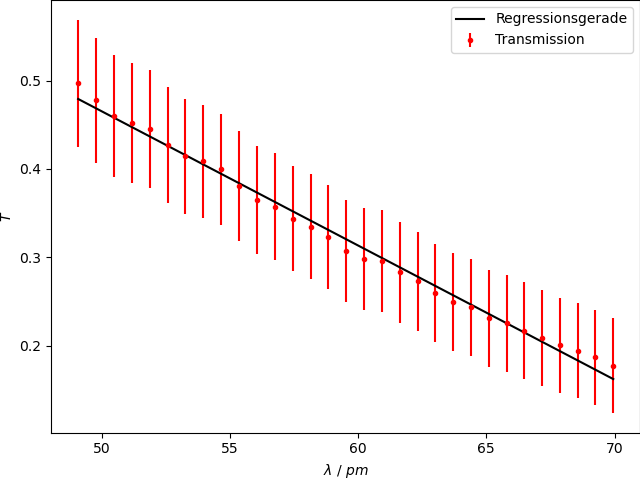
\includegraphics[height=80mm]{bilder/Transmission.png}
    \caption{Lineare Regression der Transmission in Abhängigkeit der Wellenlänge.\label{Abbildung4} }
\end{figure}


\begin{align}
    \intertext{Die folgende Ausgleichsgerade liefert die Parameter in Form der Funktion $T(\lambda) = m \cdot \lambda + b$}
    m = ( -0.0151 \pm 0.0003 )\,\frac{1}{\text{pm}}\notag \\
    b = ( 1.22 \pm 0.02 )\,. \notag
    \intertext{Somit erhält man für die Ausgleichsgerade die Form}
    T (\lambda) = -0.015\,\frac{1}{\text{pm}} \cdot \lambda + 1.221\,. \label{5}
    \intertext{Um die Compton-Wellenlänge zu bestimmen, muss zunächst die Transmission $T_{1} = \frac{I_{1}}{I_{0}}$ der ungestreuten Röntgenstrahlung, sowie die gestreuten Röntgenstrahlung $T_{2} = \frac{I_{2}}{I_{0}}$ bestimmt werden.
    Die Totzeit beträgt hierbei nur $\tau = 90\,\unit{\micro\second}$ und eine Totzeitkorrektur ist  nicht nötig, da die Impulse nicht viel sind und in der Zeit weitere Impuls nicht viel sind und in der Zeit keine weiteren Impulse identifiziert werden.
    Die Integrationszeit beträgt $t = 300\,\unit{\second}$.
    Die dabei gemessene Impulse lauten}
    I_{0} = 2731\,\, \text{Impulse}\notag \\
    I_{1} = 1180\,\, \text{Impulse}\notag \\
    I_{2} = 1024\,\, \text{Impulse}\notag\\
    \intertext{Somit folgt für die Transmissionen}
    T_{1} = (0.432 \pm 0.004)\notag \\
    T_{2} = (0.374 \pm 0.003)\,.\notag
    \intertext{Anschließend werden die Wellenlängen $\lambda_{2}$ und $\lambda_{1}$ bestimmt, indem die Transmission in die Ausgleichsfunktion (\ref{5}) eingesetzt und nach der Wellenlänge $\lambda$ umgeformt wird: }
    \lambda_{i} = \frac{T_{i} - \text{A}}{\text{B}}\notag
    \intertext{Die Compton Wellenlänge setzt sich aus der Differenz der beiden Wellenlänge $\lambda_{2}$ und $\lambda_{1}$. 
    Daraus ergibt}
    \lambda_{c} = ( 3.775 \pm 0.082 )\,\text{pm}\,.\notag
\end{align}

\notag